% Revised and extended version of Chauhan & Hegde, DATA 2026, for Springer CCIS.
% Build: pdflatex main && bibtex main && pdflatex main && pdflatex main
\documentclass[runningheads]{llncs}
\usepackage[T1]{fontenc}
\usepackage{newtxtext}
\usepackage[varvw]{newtxmath}
\usepackage{graphicx}
\usepackage{booktabs}
\usepackage{multirow}
\usepackage{url}
\usepackage{bbding}
\usepackage{color}
\renewcommand\UrlFont{\color{blue}\rmfamily}
\urlstyle{rm}

\begin{document}

\title{When Does Chunking Matter? A Three-Regime Variance Decomposition of Segmentation Effects in Retrieval-Augmented Generation\thanks{This paper is a revised and extended version of ``Chunking Is Not the Bottleneck: Why RAG Evaluation Must Look Beyond Segmentation Strategy'' presented at DATA 2026~\cite{chauhan2026chunking}. See Sect.~\ref{sec:whatsnew} for a summary of the extensions. This chapter was prepared with the assistance of AI; see the disclosure at the end of the chapter for details.}}
\titlerunning{When Does Chunking Matter?}

\author{Aaditya Chauhan\inst{1}\textsuperscript{(\Envelope)}\orcidID{0009-0000-8652-0071} \and
Nivas Hegde\inst{1}\orcidID{0009-0007-2895-6644}}
\authorrunning{A. Chauhan and N. Hegde}
\institute{Independent Researcher, U.S.A.\\
\email{aadityc28@gmail.com}, \email{nivas25h@gmail.com}}

\maketitle

\begin{abstract}
Practitioners building retrieval-augmented generation (RAG) systems devote considerable effort to choosing a text-chunking strategy. In earlier work we showed, with a balanced factorial experiment on Natural Questions and MS-MARCO, that chunking strategy explains only 1--2\% of the variance in retrieval quality and is not statistically significant. This article asks \emph{when} chunking matters. We repeat the variance-decomposition design on two further corpus regimes with span-level relevance labels: 24 technical documents from eight domains (576 core configurations) and the four legal sub-benchmarks of LegalBench-RAG (96 core configurations), adding a third embedding model. Chunking's share of variance is regime-dependent: 4.5--8\% and highly significant on technical documentation, below 1\% on legal documents, where the sub-benchmark itself explains 80--91\% of variance. Within individual corpora the median share is 20\% for technical documents against 8\% for legal ones, and the strategy-by-corpus interaction is significant on every metric. Across the 28 new corpora, the density of machine-readable (Markdown-style) section headings is associated with the size of the chunking effect ($\rho = 0.59$), whereas document length is not. A legal-aware parser that detects section structure in 81\% of the legal files does not make structure-aware chunking competitive there. An ablation separates boundary placement from heading-prefix metadata, and in an end-to-end evaluation with an LLM judge answer correctness on technical documents differs across strategies by at most a quarter of a point on a five-point scale. We argue that RAG benchmarks should report variance decomposition, interaction effects and corpus structure alongside absolute scores.

\keywords{Retrieval-augmented generation \and Text chunking \and Variance decomposition \and Benchmark evaluation \and Embedding models \and Legal document retrieval.}
\end{abstract}

\section{Introduction}
\label{sec:intro}

Retrieval-augmented generation (RAG) grounds a large language model (LLM) in external documents by retrieving passages at query time and placing them in the model's context~\cite{lewis2020rag,gao2023survey}. Before anything can be retrieved, documents must be segmented into retrieval units, and this chunking step has become one of the most discussed design decisions in the RAG ecosystem. Framework documentation~\cite{langchain2023,llamaindex2023}, tutorials~\cite{kamradt2023}, and a growing body of papers~\cite{jimenoyepes2024financial,qu2025semantic,duarte2024lumberchunker,zhao2024metachunking} compare fixed-size, sentence-based, recursive, semantic, and structure-aware splitters, and the engineering folklore holds that getting chunk boundaries right is essential.

In the conference version of this work~\cite{chauhan2026chunking} we tested that folklore with a controlled experiment. Crossing four chunking strategies, two embedding models, two chunk sizes and two established question-answering (QA) datasets, and decomposing the variance of six retrieval metrics with a Type III analysis of variance (ANOVA), we found that chunking strategy accounted for only 1--2\% of total variance and was not statistically significant, while dataset identity (24--78\%) and embedding model (11--50\%) dominated. An end-to-end evaluation with an LLM judge showed that the small retrieval differences did not propagate to answer quality. We concluded that, for factoid QA over general-purpose natural-language corpora, chunking is a low-variance factor and that the community's attention to it was disproportionate.

That conclusion was deliberately bounded. The conference paper listed settings in which chunking might matter more, including very long documents, strongly structured content, and non-QA tasks, but tested none of them. Several studies published since then make the question urgent, because they disagree with one another: some report that simple chunking is sufficient~\cite{bennani2026systematic,caspari2026complex,kreileder2026academic,li2025enhancing}, while others report that the right chunker nearly doubles retrieval quality~\cite{shaukat2026systematic} or doubles character recall on legal contracts~\cite{singh2026strucchunk}. Absolute metric comparisons on different corpora cannot resolve this disagreement. A variance decomposition that holds the design fixed and varies the corpus regime can.

\paragraph{Research question.} \emph{Under what corpus conditions does chunking strategy become a high-variance factor in RAG retrieval, and what property of a corpus predicts it?}

\paragraph{Approach.} We keep the conference paper's factorial design and statistical analysis and apply them to two new regimes chosen to probe the predictions of the original Sect.~4.3: (R2) 24 structured technical documents across eight domains, with evidence passages located as exact character spans; and (R3) the four sub-benchmarks of LegalBench-RAG~\cite{pipitone2024legalbenchrag}, about 80 million characters of legal documents with expert-annotated gold spans. Both new regimes use three embedding models rather than two. Together with the conference results (R1), this yields a three-regime map of chunking's importance built from 896 configurations. We then (i) test the regime dependence formally with strategy-by-regime and strategy-by-corpus interaction terms, bootstrap confidence intervals and multiple-comparison correction; (ii) regress the per-corpus chunking effect on corpus features to identify what drives it; (iii) separate boundary placement from metadata enrichment with a no-prefix ablation on both new regimes; (iv) add a legal-aware structure parser after discovering that our Markdown-based structure-aware chunker finds almost no structure in plain-text legal documents; (v) measure how relevance-label rigour changes the apparent size of the chunking effect; and (vi) test with an end-to-end LLM-judge evaluation whether the retrieval-stage effect on technical documents reaches the generated answer.

\paragraph{Findings.} Chunking's share of variance differs by regime: 1--2\% in general QA (not significant), 4.5--8\% on technical documentation ($p<10^{-18}$ on every metric), and below 1\% on legal documents (not significant after Holm correction except for context precision). Because the pooled share in the legal regime is depressed by the very large differences between its sub-benchmarks, we also report within-corpus shares: a median of 20\% of MRR variance for technical documents against 8\% for legal sub-benchmarks. The strategy-by-corpus interaction is significant on every metric (1.5--3.5\% of pooled variance). Of the corpus features we tested, heading density is the one associated with the chunking effect ($\rho=0.59$, $p=0.001$); document length is not ($\rho=0.10$). Structure-aware chunking is on average the best strategy on technical documents (Cliff's $\delta=0.37$ against fixed-size) and worse than fixed windows on legal documents, even with a parser that recognises legal section markers. At the retrieval stage on technical documents both structural boundaries and the heading-path prefix contribute, boundaries more. End to end, answer correctness differs across strategies by at most a quarter of a point on a five-point scale. Scoring identical retrieval runs with loose word-overlap labels instead of exact spans raises absolute scores by five to eight points but shrinks the measured chunking effect by 11--37\%, depending on the metric.

\paragraph{Contributions.} Relative to the conference paper, this article contributes: (1) two new corpus regimes and 864 new configurations, with a third embedding model; (2) a formal test of the corpus and regime dependence of chunking effects via interaction terms, within-corpus effect sizes and confidence intervals; (3) a corpus-level predictor, heading density, that practitioners can compute before running any experiment; (4) a boundary-versus-metadata ablation replicated beyond Natural Questions; (5) a legal-aware structure parser and the observation that a Markdown-based structure-aware chunker silently degenerates to recursive splitting on plain-text legal documents; (6) a measured account of how fuzzy versus exact relevance labels change conclusions about chunking; and (7) an end-to-end generation evaluation on technical documents.

\subsection{Relation to the Conference Version}
\label{sec:whatsnew}
% INSTICC requires an explicit statement of the differences. Keep this subsection.
The conference paper~\cite{chauhan2026chunking} reported the R1 experiment (32 configurations), a 2$\times$2 heading-prefix ablation on Natural Questions, and an end-to-end LLM-judge evaluation. All of that material is summarised here in Sect.~\ref{sec:r1} with citation and is not repeated in detail. Everything in Sects.~\ref{sec:design}--\ref{sec:discussion} concerning regimes R2 and R3, the interaction analysis, the corpus-feature regression, the legal-aware parser, the replicated ablation, the label-rigour comparison and the end-to-end evaluation on technical documents is new. The title, abstract, discussion and conclusions have been rewritten to reflect the new research question. The manuscript is about 60\% longer than the conference paper; roughly 85\% of the text, all figures except the R1 panel of Fig.~\ref{fig:regimes}, and all tables except the R1 column of Table~\ref{tab:regimes} are new.

\section{Background and Related Work}
\label{sec:related}

\subsection{Chunking in the RAG Pipeline}
A RAG pipeline ingests documents, segments them, embeds the segments, retrieves the nearest segments for a query and conditions a generator on them~\cite{lewis2020rag,karpukhin2020dpr}. Segmentation for retrieval predates RAG: TextTiling detected topic boundaries three decades ago~\cite{hearst1997texttiling}. Contemporary toolkits expose fixed-size splitting at token intervals, overlap windows, sentence and recursive delimiter splitting~\cite{langchain2023}, semantic splitting at embedding-similarity drops~\cite{kamradt2023}, and structure-aware splitting that follows headings and typically prepends the heading path to each chunk. More recent proposals move the problem into the model: late chunking pools chunk vectors from a document-level encoding~\cite{gunther2024latechunking}, contextual retrieval prepends an LLM-written summary of the surrounding document~\cite{anthropic2024contextual}, Meta-Chunking and LumberChunker let an LLM choose boundaries~\cite{zhao2024metachunking,duarte2024lumberchunker}, and proposition-level retrieval reduces the unit to atomic facts~\cite{chen2024densex}. Contextual training of embedders has been shown to make retrieval robust to sub-optimal chunking~\cite{conti2025conteb}, which already hints that representation and segmentation are substitutes rather than independent levers.

\subsection{Empirical Evaluations of Chunking}
Evaluations disagree sharply, and the disagreement tracks corpus and labelling choices. On general QA and academic text, semantic and LLM-based chunkers rarely beat simple baselines~\cite{qu2025semantic,bennani2026systematic,kreileder2026academic,caspari2026complex,li2025enhancing}; a large multi-objective study at CIKM 2026 finds that the winning chunker depends on the embedding model and dataset~\cite{caspari2026complex}. On financial filings, technical manuals, clinical guidelines and industrial documents, structure-aware or adaptive chunking is reported to help substantially~\cite{jimenoyepes2024financial,taiwo2026oilgas,gomezcabello2025clinical,demoura2026adaptive}. The largest contrary result, 36 strategies across six domains with LLM-graded relevance, reports paragraph-group chunking nearly doubling NDCG@5 over character chunking~\cite{shaukat2026systematic}. On contracts, StrucChunk reports that clause-aligned chunking combined with cross-reference resolution and hybrid retrieval doubles character recall on LegalBench-RAG~\cite{singh2026strucchunk}, while the benchmark's own authors found a recursive splitter better than naive fixed chunks only at the top ranks~\cite{pipitone2024legalbenchrag}. Evaluations of chunk \emph{size} likewise find the optimum dataset-dependent~\cite{bhat2025chunksize,smith2024chroma}. HiChunk argues that benchmarks with sparse evidence, such as Natural Questions, cannot discriminate chunkers at all~\cite{lu2025hichunk}, and a recent ablation of title-chain prefixes shows that LLM judges lose agreement when contextual prefixes are removed~\cite{yang2026titlechain}.

\subsection{Factor Importance in RAG}
Systematic sweeps of RAG configurations exist~\cite{wang2024bestpractices,li2025enhancing,hsia2025ragged} and generally find that reader robustness and retriever choice dominate, with chunk settings secondary; downstream quality has been shown to saturate once retrieval recall passes roughly one half~\cite{leto2024optimal}, and long-context readers degrade when evidence sits mid-context~\cite{liu2024lost}. Benchmarks such as BEIR, RAGAS, ARES and the RAG benchmark of Chen et al.~\cite{thakur2021beir,es2024ragas,saadfalcon2024ares,chen2024benchmarking} report absolute scores per configuration. To our knowledge, the conference version of this work~\cite{chauhan2026chunking} was the first to report a factorial variance decomposition of chunking against embedding model, chunk size and corpus; one clinical study has since reported $\eta^2 = 0.11$ for chunking in a one-way ANOVA~\cite{gomezcabello2025clinical}, a figure we compare against our regimes in Sect.~\ref{sec:discussion}. What has been missing is a single design run across regimes that can say \emph{where} the contradictory results come from.

\section{Experimental Design}
\label{sec:design}

\subsection{Common Factorial Design and Analysis}
All three regimes share the factorial structure of~\cite{chauhan2026chunking}: chunking strategy $\times$ chunk size $\times$ embedding model $\times$ corpus, fully crossed and balanced. The four core strategies are fixed-size token splitting, fixed-size with 20\% overlap, structure-aware splitting at Markdown headings with the heading path prepended as a bracketed prefix, and semantic splitting at embedding-similarity breakpoints~\cite{kamradt2023}. Chunk sizes are 256 and 512 tokens (cl100k tokenizer). R1 used BGE-large-en-v1.5~\cite{xiao2023cpack} and all-MiniLM-L6-v2~\cite{reimers2019sbert}; R2 and R3 add nomic-embed-text-v1.5~\cite{nussbaum2024nomic}. Retrieval uses one shared FAISS index~\cite{johnson2021faiss} over all chunks of a corpus (cosine similarity on L2-normalised vectors); this is a multi-document index in R1 and R3 and a single-document index in R2, where each corpus is one long document. Metrics are Hit@\{1,3,5\}, mean reciprocal rank (MRR)~\cite{craswell2009mrr}, normalised discounted cumulative gain (NDCG@5)~\cite{jarvelin2002ndcg} and context precision~\cite{es2024ragas}, a rank-weighted precision over the top five chunks; R3 adds Hit@\{10,20\} and recall@\{5,10,20\} over gold snippets.

Variance is decomposed with a Type III ANOVA on the main-effects model, reporting classical $\eta^2$, each factor's share of the total sum of squares~\cite{richardson2011,lakens2013}; in a balanced design Type I, II and III sums of squares coincide. Classical $\eta^2$ for one factor shrinks when another factor, here the corpus, accounts for most of the variance, so shares are not directly comparable between regimes with different between-corpus spread. We therefore also report partial $\eta^2$~\cite{richardson2011} and a within-corpus $\eta^2$, obtained by fitting strategy, chunk size and model separately inside each corpus. Interactions are tested by nested-model comparison: the increase in explained sum of squares when a strategy-by-corpus or strategy-by-regime term is added to the main-effects model, with the corresponding $F$ test. We use this formulation because corpus is nested within regime and the pooled design is unbalanced~\cite{langsrud2003}. Also new to this article are percentile bootstrap confidence intervals for $\eta^2$ from 1,000 resamples of cells within each corpus~\cite{efron1986bootstrap}, Holm correction across the six metrics~\cite{holm1979}, and, for pairwise strategy contrasts, Cliff's $\delta$~\cite{cliff1993} between the two sets of configurations together with Wilcoxon signed-rank tests paired on (corpus, chunk size, model). Where the same questions are scored under every strategy we use the Friedman test~\cite{demsar2006}.

\subsection{R1: General-Purpose QA (Conference Experiment)}
\label{sec:r1}
R1 is summarised from~\cite{chauhan2026chunking}. Five hundred queries each were drawn with a fixed seed from the Natural Questions development set~\cite{kwiatkowski2019nq}, restricted to single short-answer questions, and from the MS-MARCO passage-ranking development set~\cite{nguyen2016msmarco}; relevance used gold labels (answer-span containment and qrels respectively). The $4\times2\times2\times2=32$ configurations gave the $\eta^2$ values reproduced in the R1 column of Table~\ref{tab:regimes}, which are taken from Table~1 of the conference paper. Strategy was not significant on any metric ($F(3,25)\le 1.60$, $p>0.21$).

\subsection{R2: Structured Technical Documentation}
\label{sec:r2}
The second regime comprises 24 publicly available technical documents in eight domains (hardware manuals, cloud API documentation, software manuals, engineering specifications, technical standards, medical guidelines, legal and regulatory texts, and corporate-finance documents), three per domain, between 70 thousand and 390 thousand characters each. Each document is its own corpus. The 2,406 question--answer pairs were generated with an LLM from document segments, each with an evidence passage quoted from the source, and filtered automatically so that the quoted evidence occurs in the document; they were not verified by human annotators. Nineteen of the documents carry explicit Markdown-style headings; five (GDPR, the Basel III framework, two 10-K filings and one hardware manual; the points at zero heading density in Fig.~\ref{fig:density}) carry none, which later proves informative.

Relevance labelling was redesigned relative to the heuristic used when this corpus was first assembled. The evidence passage of each question is located as an exact character span in a whitespace-normalised copy of the document (2,229 of 2,406 pairs locate; the remainder are excluded from all strategies alike), each retrieved chunk is likewise mapped to its span after stripping any heading prefix, and a chunk is relevant if it covers at least half of the evidence span. Chunks whose text cannot be located in the document after tokenizer round-tripping can never be scored as relevant; this affects 0.2--0.6\% of chunks for the fixed-size and structure-aware chunkers and 2.3\% for semantic chunking (18\% on one document), a small bias against semantic chunking. Because the retrieval runs are identical, we also score every run with the original fuzzy word-overlap labels (at least 70\% of evidence words present in the chunk), which gives a controlled measurement of how label rigour changes conclusions (Sect.~\ref{sec:labels}). The design is $4\times2\times3\times24=576$ configurations, plus 144 configurations of a fifth, no-prefix strategy used only for the ablation in Sect.~\ref{sec:ablation}.

\subsection{R3: Legal Documents}
\label{sec:r3}
The third regime uses LegalBench-RAG~\cite{pipitone2024legalbenchrag}, which repurposes four expert-annotated legal datasets as retrieval benchmarks with exact character-span gold snippets: PrivacyQA~\cite{ravichander2019privacyqa} (194 queries over 7 privacy policies), ContractNLI~\cite{koreeda2021contractnli} (977 queries, 95 non-disclosure agreements), CUAD~\cite{hendrycks2021cuad} (4,042 queries, 462 commercial contracts) and MAUD~\cite{wang2023maud} (1,676 queries, 150 merger agreements). Documents average 11 thousand characters in ContractNLI, 25 thousand in PrivacyQA, 56 thousand in CUAD and 351 thousand in MAUD, so only MAUD is as long as the R2 documents. Each sub-benchmark is indexed as one corpus, so a query must find the right passage among all documents in the set. Gold spans are mapped exactly into normalised space; NDCG credits each distinct gold snippet once, since 35\% of queries have several. The core design is $4\times2\times3\times4=96$ configurations.

Running the generic structure-aware chunker on these documents revealed that only 2 of the 714 files contain a Markdown heading, so on all the others the chunker fell back to recursive delimiter splitting without any prefix. We therefore added a \emph{legal-aware} variant that first promotes conventional contract markers (``ARTICLE II'', ``Section 5.3 Title.'', ``1. DEFINITIONS.'' and all-capital title lines) to headings and then applies the unchanged structure-aware algorithm, and its no-prefix twin. Only heading lines are lifted into the heading path, so chunk text remains verbatim document text and span evaluation is unaffected (99.4\% of chunks locate). These two strategies add 48 configurations, for 144 in total.

\section{Results}
\label{sec:results}

\subsection{Chunking's Share of Variance Across Regimes}
\label{sec:regimes}
Table~\ref{tab:regimes} and Fig.~\ref{fig:regimes} place the three regimes side by side. In R2, chunking strategy explains 4.5--8.2\% of the variance in the five ranking metrics, with $F(3,\,546)\ge 32.5$ and $p<10^{-18}$ on every metric; the bootstrap intervals exclude the general-QA point values. For context precision the share is 25\%, but that figure is driven by fixed-size chunking with overlap, whose near-duplicate neighbouring chunks are both counted as relevant (mean context precision 0.183 against 0.152--0.164 for the other strategies); without the overlap strategy the share is 6.9\%, in line with the ranking metrics. In R3 the pooled strategy share is 0.3--0.7\%, with bootstrap upper limits of 0.9--2.7\% that reach the general-QA range (0.9--2.0\%) but contain the R1 point value only for Hit@1, and the sub-benchmark explains 80--91\% of variance. The only Holm-significant R3 effect, on context precision, is again due to the overlap strategy and disappears without it ($p=0.13$). Among the other factors, the corpus is always the largest (34--45\% in R2). The embedding model is second in R2 (18--24\%) but shrinks to 0.5--2.5\% in R3, where it is comparable to or smaller than chunk size (2--5\% in R3, 3--4\% in R2).

The pooled R3 share is small partly because the four sub-benchmarks differ enormously in difficulty, which inflates the total variance against which every design factor is measured. Two measures that remove this dependence give a less extreme but consistent contrast. Partial $\eta^2$ for strategy is 15--23\% on the ranking metrics in R2 against 3--7\% in R3. The within-corpus share of MRR variance has a median of 20\% over the 24 technical documents (interquartile range 13--27\%) against 1.4\%, 6.5\%, 9.4\% and 10.6\% for ContractNLI, MAUD, CUAD and PrivacyQA (median 8\%; Mann--Whitney $p=0.02$ for MRR, $0.07$ for NDCG@5, $0.21$ for Hit@5). Depending on the metric and the measure, chunking therefore matters roughly two to five times more on the technical documents than on the legal ones (the within-corpus contrast is significant for MRR only), rather than the factor of ten or more that the pooled shares alone would suggest.

\begin{figure}[t]
\centering
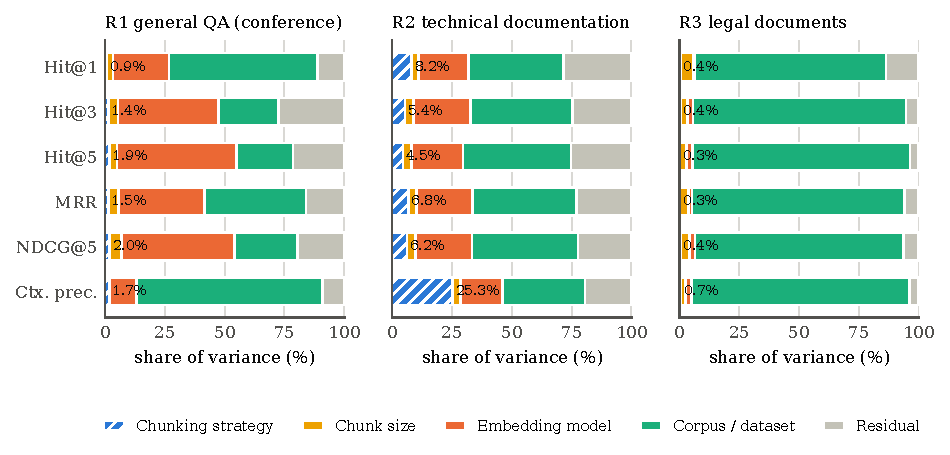
\includegraphics[width=\textwidth]{figs/fig_regimes_eta2.pdf}
\Description{Three panels of horizontal stacked bars, one per corpus regime, showing for each of six retrieval metrics how total variance divides between chunking strategy, chunk size, embedding model, corpus and residual. The chunking-strategy segment is hatched and labelled; it is 1 to 2 percent in general QA, 4.5 to 25 percent in technical documentation, and below 1 percent in legal documents.}
\caption{Variance decomposition ($\eta^2$) per metric in the three regimes. The hatched segment is chunking strategy. R1 panel reproduced from the data of~\cite{chauhan2026chunking}, Table~1.}
\label{fig:regimes}
\end{figure}

\begin{table}[t]
\caption{Share of variance ($\eta^2$, \%) explained by chunking strategy in each regime, with 95\% bootstrap confidence intervals and Holm-corrected significance. R1 values are reproduced from Table~1 of~\cite{chauhan2026chunking}.}
\label{tab:regimes}
\centering
\small
\setlength{\tabcolsep}{4pt}
\begin{tabular}{lccc}
\toprule
Metric & R1 general QA & R2 technical docs & R3 legal docs \\
 & ($n=32$) & ($n=576$) & ($n=96$) \\
\midrule
Hit@1 & 0.9 (n.s.) & 8.2 [6.0, 10.6]$^{***}$ & 0.4 [0.1, 2.7] (n.s.) \\
Hit@3 & 1.4 (n.s.) & 5.4 [3.6, 7.0]$^{***}$ & 0.4 [0.1, 1.4] (n.s.) \\
Hit@5 & 1.9 (n.s.) & 4.5 [3.1, 6.3]$^{***}$ & 0.3 [0.0, 0.9] (n.s.) \\
MRR & 1.5 (n.s.) & 6.8 [4.9, 8.6]$^{***}$ & 0.3 [0.0, 1.3] (n.s.) \\
NDCG@5 & 2.0 (n.s.) & 6.2 [4.4, 8.1]$^{***}$ & 0.4 [0.1, 1.5] (n.s.) \\
Context precision & 1.7 (n.s.) & 25.3 [21.0, 28.7]$^{***}$ & 0.7 [0.2, 1.6]$^{*}$ \\
\bottomrule
\end{tabular}
\\[2pt]{\footnotesize $^{***}p_{\mathrm{Holm}}<0.001$; $^{*}p_{\mathrm{Holm}}<0.05$; n.s.\ not significant.}
\end{table}


\subsection{Chunking Effects Depend on the Corpus}
\label{sec:interaction}
Pooling the 672 core configurations of R2 and R3 and adding a strategy-by-corpus interaction to the main-effects model increases the explained share of total variance by 1.5--3.5\% depending on the metric (81 degrees of freedom; $p<10^{-4}$ on every metric), which is larger than the pooled main effect of strategy on the five ranking metrics (0.8--2.2\%). The effect of chunking strategy thus depends on the corpus. The coarser strategy-by-regime contrast, which asks only whether the pattern differs between technical and legal documents, accounts for 0.2--0.5\% (3 degrees of freedom; $p<10^{-3}$ on every metric): it is statistically reliable but explains only about a seventh of the corpus-level interaction, so most of the heterogeneity lies between individual corpora rather than between the two regimes. Within R2, strategy is Holm-significant on all six metrics ($p_{\mathrm{Holm}}<10^{-18}$); within R3 on none except context precision ($p_{\mathrm{Holm}}=0.02$; see above). R1 is not part of the pooled model because it used two rather than three embedding models and a separate pipeline.

\subsection{Which Strategy Wins Depends on the Regime}
\label{sec:pairwise}
On technical documents structure-aware chunking is on average better than every alternative (Cliff's $\delta$ against fixed-size $0.37$, against fixed-overlap $0.24$, against semantic $0.31$; all paired Wilcoxon $p<10^{-4}$, $n=144$ pairs), and fixed-overlap beats plain fixed-size ($\delta=0.16$). The average hides variation: structure-aware has the best mean MRR on 16 of the 24 documents, fixed-overlap on four, semantic on three and fixed-size on one. On legal documents the generic structure-aware chunker, which here degenerates to recursive splitting, is worse than fixed-size ($p<0.001$) and fixed-overlap ($p=0.001$) on MRR; semantic chunking is worse than fixed-size ($p=0.02$) but not reliably worse than fixed-overlap ($p=0.10$) (Table~\ref{tab:legal}).

The legal-aware parser does not change this picture. It detects section structure in 578 of the 714 legal files (81\%: 99\% of merger agreements, 85\% of non-disclosure agreements, 75\% of CUAD contracts, but only 2 of the 7 privacy policies), so the comparison is now a genuine test of structure-aware chunking rather than of a fallback. Yet clause-aligned boundaries lower MRR relative to fixed-size windows on every sub-benchmark except MAUD, where all strategies are near zero and the legal-aware variant is nominally the best: pooled over the 24 paired cells, the boundary effect is $-0.026$ MRR ($p=0.0006$) and adding the heading-path prefix recovers only $+0.002$ ($p=0.18$). Substituting the legal-aware chunker for the generic one in the R3 decomposition leaves chunking's pooled share at 0.3--0.7\% (uncorrected $p=0.04$ for Hit@3 and $p=0.002$ for context precision; no ranking metric survives Holm correction). One reading, which we have not tested directly, is that contract clauses are long relative to the gold snippets (mean gold span 320--710 characters), so section-aligned chunks dilute the relevant sentence in more surrounding text than a fixed window does; what the heading prefix adds in topical context, the longer chunk loses in precision.

\begin{table}[t]
\caption{R3 legal documents: mean MRR per strategy and sub-benchmark (6 cells each: 2 chunk sizes $\times$ 3 models), and the fraction of files in which the legal-aware parser detected section structure. Generic structure-aware chunking detected structure in 2 of the 714 files and otherwise fell back to recursive splitting.}
\label{tab:legal}
\centering
\footnotesize
\setlength{\tabcolsep}{3.5pt}
\begin{tabular}{lcccccc}
\toprule
Benchmark & Fixed & Fixed-ovl. & Semantic & Struct.\ (generic) & Struct.\ (legal) & Struct.\ files \\
\midrule
PrivacyQA   & 0.505 & 0.496 & 0.447 & 0.473 & 0.470 & 29\% \\
ContractNLI & 0.235 & 0.246 & 0.234 & 0.217 & 0.195 & 85\% \\
CUAD        & 0.211 & 0.218 & 0.193 & 0.199 & 0.186 & 75\% \\
MAUD        & 0.023 & 0.027 & 0.027 & 0.022 & 0.028 & 99\% \\
\midrule
All (24 cells) & 0.243 & 0.247 & 0.225 & 0.228 & 0.220 & 81\% \\
\bottomrule
\end{tabular}
\end{table}

\subsection{What Predicts the Size of the Chunking Effect}
\label{sec:features}
\begin{figure}[t]
\centering
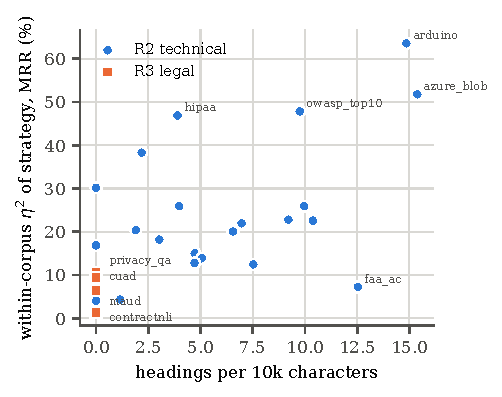
\includegraphics[width=0.62\textwidth]{figs/fig_heading_density.pdf}
\Description{Scatter plot of 28 corpora. Horizontal axis: Markdown headings per ten thousand characters, from 0 to about 15. Vertical axis: within-corpus share of MRR variance explained by chunking strategy, from 0 to 65 percent. Technical documents are circles and rise with heading density; the four legal sub-benchmarks are squares at zero heading density with variance shares between 1 and 11 percent.}
\caption{Per-corpus chunking effect against heading density for the 24 technical corpora (circles) and 4 legal sub-benchmarks (squares). Spearman $\rho=0.59$, $p=0.001$.}
\label{fig:density}
\end{figure}
For each of the 28 new corpora we fit the within-corpus ANOVA (strategy, size, model; 24 cells) on MRR and relate chunking's within-corpus $\eta^2$ to three corpus features (Fig.~\ref{fig:density}). Heading density (Markdown headings per 10 thousand characters) correlates with the chunking effect at Spearman $\rho=0.59$ ($p=0.001$) and with the structure-aware advantage over fixed-size at $\rho=0.72$ ($p<0.001$). Mean document length does not correlate with the chunking effect ($\rho=0.10$, $p=0.63$), and neither does evidence-span length ($\rho=-0.20$, $p=0.30$), although longer evidence spans go with a smaller structure-aware advantage ($\rho=-0.44$, $p=0.02$). In a joint linear model of the three features heading density is the only significant predictor ($p=0.002$; adjusted $R^2=0.32$); the association also holds within R2 alone ($\rho=0.47$, $p=0.02$; regression $p=0.005$). The relationship is far from deterministic: one heading-free 10-K filing has a within-corpus share of 30\%, and one document with 12.5 headings per 10 thousand characters has a share of 7\%. Easier corpora (higher mean Hit@5) tend to show a larger structure-aware advantage ($\rho=0.61$, $p<0.001$) and a weakly larger chunking share ($\rho=0.35$, $p=0.07$), which motivates the floor-effect check that follows.

\subsection{Floor-Effect Check for the Legal Regime}
\label{sec:floor}
Absolute span-level performance on the legal documents is low (mean Hit@5 0.35; 0.04 on MAUD) even though document-level Hit@5 is higher (0.62 on ContractNLI, 0.81 on MAUD, 0.98--0.99 on PrivacyQA and CUAD): retrieval usually finds the right document but not the right passage. A floor effect is therefore a competing explanation for the small $\eta^2$. We checked it in four ways. Excluding MAUD raises chunking's share to 0.7--1.5\% (Hit@5 $p=0.048$); excluding both MAUD and ContractNLI, which leaves 48 cells at mean Hit@5 0.53, raises it to 1.1--2.4\% (Hit@5 $p=0.024$), reaching the general-QA level but remaining three to eight times below R2 on the ranking metrics. Within PrivacyQA alone, where Hit@5 is 0.71, chunking's within-corpus share of MRR variance (11\%) is below the R2 median (20\%). Finally, at retrieval depths where the metric is no longer near floor, the gap persists: mean Hit@20 is 0.50 and recall@20 over gold snippets is 0.41, yet chunking explains only 0.1\% of Hit@20 variance and 0.3\% of recall@20 variance (strategy $p=0.10$ and $p=0.02$), while the sub-benchmark explains over 90\%. The regime difference thus survives the floor-effect check in direction, although part of the smallness of the pooled R3 estimate is attributable to task difficulty and to the between-sub-benchmark spread discussed in Sect.~\ref{sec:regimes}; the within-corpus contrast (20\% against 8\%) is the more conservative summary.

\subsection{Boundaries Versus Metadata: The Prefix Ablation Replicated}
\label{sec:ablation}
Structure-aware chunkers do two things at once: they cut at structural boundaries and they prepend the heading path to each chunk. The conference paper separated the two on Natural Questions with a $2\times2$ ablation and found both effects small (boundaries $-0.034$ MRR, prefix $+0.004$; four cells per condition, no significance claimed). We run a three-condition version on both new regimes by adding a no-prefix variant with identical boundaries (Fig.~\ref{fig:ablation}). On technical documents (144 paired cells) both components help and both are significant: structural boundaries alone raise MRR from 0.588 to 0.634 ($+0.045$, Wilcoxon $p<10^{-13}$) and the prefix adds a further $+0.020$ ($p<10^{-7}$), so boundary placement carries about 70\% of the retrieval-stage gain. The split depends on whether structure exists: on the 30 cells from the five heading-free technical documents, the no-prefix variant (which there reduces to recursive splitting) still gains $+0.036$ over fixed-size, but the prefix adds nothing because there is no heading to prepend. On legal documents with the legal-aware parser (24 paired cells) the boundary effect is negative ($-0.026$, $p<0.001$) and the prefix effect is nil ($+0.002$, $p=0.18$). Taken together with R1, the ablation yields three different answers in three regimes, which is itself the point: neither ``structure-aware chunking helps'' nor ``the gain is only metadata'' is a general statement. Whether the same split holds at the generation stage cannot be settled with our end-to-end sample (Sect.~\ref{sec:generation}).

\begin{figure}[t]
\centering
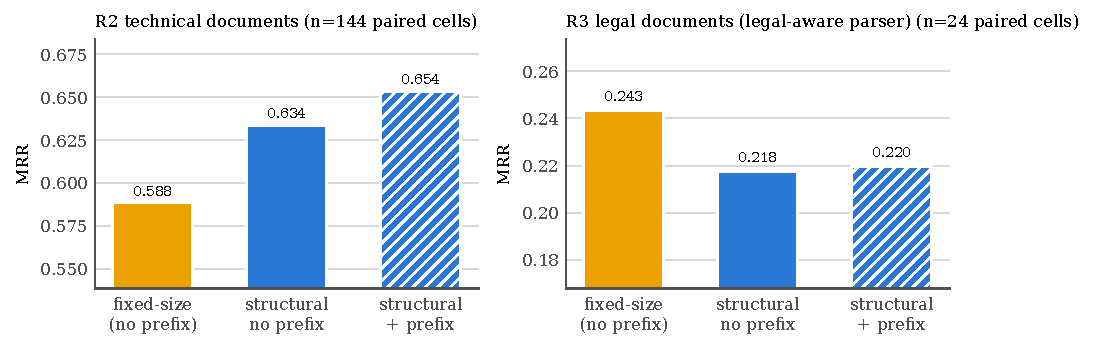
\includegraphics[width=\textwidth]{figs/fig_prefix_ablation.pdf}
\Description{Two bar charts of mean MRR for three conditions: fixed-size without prefix, structural boundaries without prefix, structural boundaries with heading prefix. Left panel, technical documents: bars rise from 0.588 to 0.634 to 0.654. Right panel, legal documents with the legal-aware parser: bars fall from 0.243 to 0.218 and recover slightly to 0.220.}
\caption{Boundary-versus-prefix ablation on R2 technical documents (left, 144 paired cells) and R3 legal documents with the legal-aware parser (right, 24 paired cells). Mean MRR; hatched bar includes the heading-path prefix.}
\label{fig:ablation}
\end{figure}

\subsection{Does Label Rigour Change the Answer?}
\label{sec:labels}
Scoring the identical R2 retrieval runs with the fuzzy word-overlap labels instead of exact spans raises every absolute metric by five to eight points (MRR 0.61 to 0.68) but \emph{shrinks} chunking's share of variance, to between 63\% (Hit@5) and 89\% (Hit@1) of its span-label value, and shrinks the structure-aware advantage over fixed-size on MRR from 0.065 to 0.045. Fuzzy labels inflate fixed-size and fixed-overlap scores most (+0.076 MRR) and structure-aware least (+0.056), because loose matching credits chunks that contain only part of the evidence, which fixed windows produce more often. The correlation between the two label schemes across configurations is 0.85--0.88 for the five ranking metrics and 0.52 for context precision. Loose labels therefore blur rather than manufacture strategy differences in this regime, which cautions against reading a small chunking effect under heuristic labels as evidence that chunking is irrelevant, and equally against the conference paper's implicit assumption that heuristic labels flatter structure-aware chunking.

\subsection{Does the Technical-Regime Effect Reach the Generated Answer?}
\label{sec:generation}
The conference paper showed for R1 that chunking differences do not propagate to answer quality. We repeat that test on R2, where chunking matters at the retrieval stage in the full factorial. For 200 questions sampled uniformly over the 24 technical documents we retrieve the top five chunks under each strategy (BGE-large, 512 tokens), generate an answer from the retrieved context only with a small, inexpensive LLM (Claude Haiku 4.5), and score it with a larger model as judge (Claude Opus 5) for correctness against the gold answer and faithfulness to the context, each on a 1--5 scale. Table~\ref{tab:generation} reports the results. Mean correctness ranges from 4.30 (semantic) to 4.53 (structure-aware). Because the same questions are scored under every strategy, we use the Friedman test, which indicates that the four core strategies differ ($\chi^2=8.5$, $p=0.04$). The largest contrast is between structure-aware and semantic chunking ($+0.235$, uncorrected Wilcoxon $p=0.02$), but no pairwise contrast survives Holm correction (smallest $p_{\mathrm{Holm}}=0.10$; structure-aware against fixed-size $+0.165$, uncorrected $p=0.08$). Faithfulness is at ceiling (4.94--4.95) for every strategy and does not differ ($p=0.87$), as in R1. In this configuration the retrieval-stage advantage of structure-aware chunking is itself small (MRR $+0.019$ over fixed-size on the 200 questions, $p=0.57$), so the sample has limited power to show propagation. Per question, span-label MRR and correctness correlate at $r=0.57$ over the core strategies (0.52--0.60 within each strategy), higher than the $0.28$ reported for Natural Questions; the two evaluations used different generator and judge models, so we do not interpret the difference further. The no-prefix variant scores 4.41, between fixed-size (4.37) and the full structure-aware chunker (4.53); neither step is significant on its own (boundaries $+0.040$, $p=0.70$; prefix $+0.125$, $p=0.06$), so the split of the end-to-end gain between boundaries and prefix remains open. Overall, the end-to-end strategy effect on technical documents is at most a quarter of a point on a five-point scale.

\begin{table}[t]
\caption{End-to-end evaluation on R2 technical documents (200 questions, top-5, BGE-large, 512 tokens). Correctness and faithfulness are 1--5 judge scores. Friedman test across the four core strategies: correctness $p=0.04$, faithfulness $p=0.87$.}
\label{tab:generation}
\centering
\begin{tabular}{lccc}
\toprule
Strategy & MRR & Correctness & Faithfulness \\
\midrule
Fixed-size & 0.610 & 4.37 & 4.95 \\
Fixed-overlap & 0.607 & 4.42 & 4.94 \\
Semantic & 0.611 & 4.30 & 4.95 \\
Structure-aware (with prefix) & 0.629 & 4.53 & 4.95 \\
\midrule
Ablation: structure-aware, no prefix & 0.612 & 4.41 & 4.95 \\
\bottomrule
\end{tabular}
\end{table}

\subsection{Cost}
\label{sec:cost}
Chunking cost separates the strategies far more than retrieval quality does. On the technical documents, where timings were recorded without any cache, median chunking time per document is 20\,ms for fixed-size and fixed-overlap, 139\,ms for structure-aware, and 6.7\,s for semantic chunking, which must embed every sentence before it can choose boundaries: roughly 50 times the cost of structure-aware chunking and 340 times that of fixed-size. On the legal corpora the non-semantic strategies take a median over configurations of 0.8--0.9\,s (fixed-size, fixed-overlap), 2.7\,s (generic structure-aware) and 4.6\,s (legal-aware parser) per sub-benchmark, ranging from a fraction of a second on PrivacyQA to about 20\,s on MAUD; semantic-chunking times there are not comparable because sentence embeddings were cached across restarts of the run, but uncached semantic chunking of the 53-million-character MAUD corpus took on the order of hours per configuration on a single consumer GPU. Embedding cost scales with chunk count, and the structure-aware strategies produce more chunks than fixed-size at the same target size (a median of 61\% more per configuration in R2 and 35--39\% more in R3) because sections are split at their own boundaries. Semantic chunking is not the best strategy on average in either new regime and is the most expensive wherever its cost was measured cleanly, consistent with~\cite{qu2025semantic}.

\section{Discussion}
\label{sec:discussion}

\subsection{A Map, Not a Verdict}
The conference paper's claim was that chunking is a low-variance factor for QA over general-purpose corpora; it listed very long documents among the settings where chunking might matter substantially more. The new regimes leave the first part untouched and qualify the second. Chunking strategy is a clearly non-negligible factor on technical documentation, and a small one on the legal documents, including MAUD, whose merger agreements are as long as most of the technical documents we tested. Document length is not associated with the size of the chunking effect in our data; heading density is. We do not claim that length never matters: only one of our sub-benchmarks consists of very long documents, and it is also the one closest to floor. The regimes also differ in more than structure: R2 retrieval is within a single document while R3 retrieval is across 7 to 462 documents, R2 questions were machine-generated while R3 gold spans are expert annotations, and the domains differ. The regime contrast should therefore be read as descriptive, and the heading-density relationship, which also holds within R2, as the more portable finding. The conference paper's motivating example was a team spending a week on chunking for a technical-documentation corpus; our R2 results indicate that on such a corpus the choice is not negligible, although it remains smaller than the choice of embedding model. Even in R2 the gain is bounded: chunking's pooled share of variance (4.5--8\% on ranking metrics) is roughly a fifth to a third of the embedding model's and a tenth to a fifth of the corpus's. The much larger share for context precision reflects how that metric rewards overlapping chunks rather than a retrieval advantage (Sect.~\ref{sec:regimes}).

This picture is consistent with the pattern of disagreement in the recent literature, without proving that it explains it. Studies that report small or inconsistent chunking effects mostly work on general QA and academic text~\cite{bennani2026systematic,caspari2026complex,kreileder2026academic}, and a configuration sweep likewise finds chunk settings of minor importance~\cite{li2025enhancing}. Studies that report large effects work on manuals, filings, clinical guidelines and industrial documents~\cite{taiwo2026oilgas,gomezcabello2025clinical,demoura2026adaptive,jimenoyepes2024financial}, document types that resemble the heading-rich part of our R2. The clinical study's $\eta^2$ of 0.11 for chunking~\cite{gomezcabello2025clinical} is somewhat above our pooled R2 range (4.5--8\%) and below our within-corpus median (20\%); since that study varied chunking alone on one corpus, the within-corpus figure is the closer comparison. Two results are harder to place. Shaukat et al.~\cite{shaukat2026systematic} report paragraph-group chunking nearly doubling NDCG@5 under LLM-graded relevance; our label comparison (Sect.~\ref{sec:labels}) shows that the labelling protocol alone can change the measured effect by 11--37\% even between two deterministic schemes, and one recent study reports that LLM judgments shift with the context prefixes that structure-aware chunkers add~\cite{yang2026titlechain}, so protocol differences may contribute. StrucChunk~\cite{singh2026strucchunk} doubles character recall on LegalBench-RAG with an intervention that combines clause-aligned boundaries, cross-reference resolution and hybrid lexical--dense retrieval against a 500-character baseline. Our legal-aware parser tests only a boundary component, with a different parser and embedder, and finds that it lowers MRR relative to fixed windows; this is compatible with StrucChunk's gain arising from the combination rather than from boundaries alone, but our design cannot attribute it. Both cases illustrate why absolute comparisons across corpora and protocols are hard to transfer without a variance decomposition.

\subsection{Implications for Practitioners}
The heading-density result suggests an inexpensive first check: count machine-readable section headings (in our corpora, Markdown-style headings) per ten thousand characters before running any retrieval experiment. Section markers that are visible to a reader but not marked up, such as the ``ARTICLE II'' lines of contracts, did not carry the same benefit even when a parser recovered them. In our technical corpora, documents with several headings per ten thousand characters usually, though not always, showed a sizeable chunking effect, and structure-aware chunking with heading prefixes was the best strategy on 15 of the 19 documents that have headings; a pilot comparison on one's own corpus remains necessary. On the legal corpora, none of the segmentation strategies we tested, including a rule-based domain parser, improved on fixed windows, and representation-level approaches such as contextual prefixes and late chunking~\cite{anthropic2024contextual,gunther2024latechunking,conti2025conteb} may be the more promising direction. In R1 and R2 the embedding model explains several times more variance in the ranking metrics than chunking strategy, so model selection comes first there; in R3 neither design choice explains much, and the difficulty of the sub-benchmark dominates. Semantic chunking is not the best strategy on average in R2 or R3 and was 50 to 340 times more expensive than the alternatives where we could time it cleanly (Sect.~\ref{sec:cost}), consistent with~\cite{qu2025semantic}. Finally, a team that evaluates a structure-aware chunker should verify that it actually detects structure on their corpus: ours silently fell back to recursive splitting on 712 of 714 legal files, and the fraction of documents in which structure is detected (reported as \texttt{structured\_files\_frac} in our results) is a cheap sanity check that benchmark reports should include.

\subsection{Implications for Benchmark Design}
The conference paper asked benchmark authors to report variance decomposition, effect sizes and interaction effects alongside absolute scores. The present results show why the interaction matters and add three further requests. The strategy-by-corpus interaction here is larger than the pooled main effect of strategy on the ranking metrics, so a main effect averaged over corpora says little about any one of them. First, report within-corpus or partial effect sizes in addition to pooled shares, because pooled $\eta^2$ depends on how much the corpora differ from one another. Second, report the relevance-labelling protocol and, where feasible, score the same runs under more than one protocol; in our comparison loose labels inflated absolute scores and compressed strategy differences. Third, characterise the corpus structurally, at minimum by heading density and document length, and check metrics such as context precision for sensitivity to overlapping chunks.

\subsection{Limitations}
Our study covers three regimes and 30 corpora (two in R1, 28 new), not a continuous sampling of corpus space, and the regimes differ in several respects at once (domain, document structure, single- versus multi-document index, and how the gold labels were produced), so regime-level contrasts are descriptive. The heading-density relationship is correlational, and no threshold should be read into it. The R2 questions and evidence passages were LLM-generated and automatically filtered rather than human-annotated, and each R2 corpus is a single document. We tested four core strategies and two chunk sizes; proposition-level, LLM-driven and late-chunking approaches, sizes above 512 tokens, and reranking are outside the design. Only our own Markdown-based structure-aware chunker and a regular-expression legal parser (which detects structure in 81\% of the legal files but only 2 of 7 privacy policies) were tested; a learned clause segmenter might behave differently. End-to-end generation is evaluated for R1 (conference paper) and R2 but not for R3, and the R2 evaluation uses one embedding model, one chunk size, 200 questions and a single LLM judge from the same model family as the generator, without human validation. Absolute performance in R3 is low enough that a floor effect contributes to the small pooled chunking share there. Each cell is a single deterministic run, so the variance decomposed is between-configuration variance; the bootstrap resamples cells within corpora, and because $\eta^2$ is bounded at zero its lower limits near zero are not informative. The strategy-by-regime test covers R2 and R3 only. All corpora are English.

\section{Conclusions}
\label{sec:conclusions}
Starting from the conference finding that chunking strategy explains 1--2\% of retrieval variance in general-purpose QA, we asked when it matters and applied the same balanced factorial design to two further regimes and 864 new configurations. The answer depends on the corpus. On technical documentation chunking strategy is a significant factor (4.5--8\% of pooled variance, a median of 20\% within a document), and structure-aware chunking is the best strategy on average; on legal documents it explains under 1\% of pooled variance and a median of 8\% within a sub-benchmark, and neither generic nor legal-aware structure-aware chunking improves on fixed windows. The interaction between strategy and corpus is larger than the pooled main effect of strategy on the ranking metrics, and the density of Markdown-style headings, not document length, is the corpus feature associated with a large effect. At the retrieval stage on technical documents both structural boundaries and heading prefixes contribute; end to end, answer correctness moves by at most a quarter of a point on a five-point scale. Stricter relevance labels lower absolute scores by five to eight points and enlarge, rather than shrink, the measured differences between strategies. The conference paper's recommendation stands in a qualified form: in the general-QA and technical regimes choose the embedding model first, then check whether the corpus has machine-readable structure before investing in chunking. Benchmarks that report variance decomposition, interactions, within-corpus effect sizes, the labelling protocol and corpus structure would let the community move from asking whether chunking matters to describing where it does.

\begin{credits}
\subsubsection{\ackname}
Code, the technical-document corpus with its question--answer pairs, and all per-configuration results are available at \url{https://github.com/aadityc91/TechChunkBench} (branch \texttt{ccis-extension}). LegalBench-RAG was obtained from its authors' public release~\cite{pipitone2024legalbenchrag} and is not redistributed.

\subsubsection{Disclosure of Interests}
The authors have no competing interests to declare that are relevant to the content of this article.

\subsubsection{Disclosure of AI Use}
The manuscript, or parts thereof, was drafted and edited with the assistance of artificial intelligence (AI) using Claude developed by Anthropic (Claude Fable 5.1 and 5.2, November 2026), based on the authors' experimental design, results and interpretations. Experiment code and analysis scripts used within this manuscript were written and refined with the assistance of the same tool. The generated content was carefully reviewed, verified and endorsed by the authors to ensure the accuracy and integrity of the final manuscript.
\end{credits}

\bibliographystyle{splncs04}
\bibliography{references}

\end{document}
